\textit{Portions of this chapter were originally published in collaboration with Jake VanderPlas in the September 2018 edition of the Journal of Open Source Software (Fleming and VanderPlas 2018, JOSS, Vol. 3, 29, p. 781; 2018, DOI: 10.21105/joss.00781), and are reproduced below with permission of the Journal of Open Source Software. Portions of this chapter were originally published in collaboration with Rory Barnes, Rodrigo Luger, and Jacob VanderPlas in March 2020 in the Astrophysical Journal (Fleming et al., 2020, ApJ, Vol. 891, 2; 2020 \textcopyright \ American Astronomical Society, DOI: 10.3847/1538-4357/ab77ad), and are reproduced below with permission of the American Astronomical Society.}

\

In this thesis, I have developed numerous theoretical models, all implemented in \vplanet, that simulate the long-term evolution of stars and their planets. In this Chapter, I explore how I can use those models to infer the evolutionary history of exoplanetary systems in conjunction with observational constraints using Bayesian statistics. I explain the significant numerical challenges that can make such studies intractable, motivating the development of a software package for rapid, approximate Bayesian inference, \approxposterior \citep{FlemingVanderPlas2018}. I describe the \approxposterior algorithm and implementation in detail, provide example use cases, and conclude by discussing in-progress and future work with \approxposterior. In the next Chapter, I apply the methods developed in this Chapter to infer the high-energy radiation history of the nearby planet-hosting star, TRAPPIST-1.

\section{Bayesian Inference with Computationally-Expensive Models}

I can constrain the evolutionary histories of exoplanetary systems using the models implemented in \vplanet by calibrating the simulation initial conditions such that the output agrees with the observed data, within the observational uncertainties.  This task is mathematically codified by the statistical method of Bayesian inference. Generally, Bayesian inference proceeds as follows:  One seeks to derive a probability distribution for model parameters, e.g. \vplanet parameters such as a the stellar mass or tidal Q.  That distribution should quantify how likely it is that the parameter takes on certain values and capture the inherent uncertainty in the parameter values given data.  This distribution is known as the ``posterior probability distribution" and accounts for observed data, the data uncertainties, and one's prior belief about how the parameters are distributed. To compute the posterior distribution of model parameters, \textbf{x}, given observed data, $Data$, one uses Bayes' Theorem: 
\begin{equation} \label{AP:eqn:bayes}
P(\textbf{x} | Data) \propto P(Data | \textbf{x}) P(\textbf{x}),
\end{equation}
where $P(\textbf{x} | Data)$ is the posterior probability of \textbf{x} given $Data$, $P(\textbf{x})$ is the prior probability assigned to \textbf{x}, and $P(Data | \textbf{x})$ is the probability of the data given \textbf{x}, commonly referred to as the likelihood of $Data$ given \textbf{x}. This equation neglects the normalization constant, $1/P(Data)$, as this is typically quite difficult to compute because it requires integrating the likelihood over the prior. Through Bayes' Theorem, the posterior probability can be thought of as using data to update one's prior belief of how $\textbf{x}$ is distributed, given a model for the likelihood of the data. Note that in this thesis, I use the natural logarithm of Bayes' Theorem and refer to $\ln P(\textbf{x} | Data)$ to as the ``lnprobability". For notational convenience, I define the lnprobability as $f(\textbf{x})$. 

With \vplanet, I must compute the likelihood by running a simulation to compute a prediction, e.g. a planet's orbital period after Gyrs of tidal evolution, and compare it to the observed value and associated uncertainty. This comparison is typically performed using a $\chi^2$ statistic if the uncertainties are assumed to be Gaussian and uncorrelated, a standard assumption. Since computing the likelihood requires running a \vplanet simulation and hence the posterior is not an analytic function, and since I cannot compute $P(Data)$, I must use a Monte Carlo sampling technique to estimate the posterior distribution. This procedure is usually done using Markov Chain Monte Carlo (MCMC) methods such as the affine-invariant MCMC code, \emcee, whose usage is ubiquitous in astronomy \citep{ForemanMackey2013}. MCMC methods are incredibly powerful as they just require computing a function that is proportional to the posterior probability, e.g. the likelihood times the prior for a given \textbf{x}, allowing them to neglect the normalization term and directly sample from the posterior distribution. How the sampling proceeds depends on the MCMC algorithm, but generally given long enough MCMC chains, the derived distributions are asymptotically guaranteed to converge to the correct distribution. Standard MCMC runs can therefore require upwards of $10^6$ likelihood calculations, likely more depending on the dimensionality of the problem, to draw a suitable number of samples from the posterior distribution and build up statistical power.  

Consider an experiment in which I want to infer the stellar and tidal evolution of an exoplanetary system given some observed data. \vplanet has reasonable physical models for both phenomena, so I could use \vplanet within an MCMC chain to constrain the evolution. Each \vplanet simulation with these models, however, takes one minute to run. If the MCMC chain required  $10^6$ likelihood calculations, the MCMC run would expend about 2 years of core-hours. This extreme computational expense renders MCMC sampling with \vplanet computationally intractable at scale, especially for model comparison studies that require multiple MCMC runs. Furthermore, because of the ``Curse of Dimensionality", the number of samples required to resolve the posterior distribution grows exponentially with the dimensionality of the problem \citep{Bellman1957}, exacerbating this issue for more complex simulations. Clearly, for Bayesian inference to become feasible for models like \vplanet with runtimes $\geq 10$ seconds, a method to compute the posterior distribution while minimizing the number of forward model evaluations is required. I address this issue and enable Bayesian parameter inference with \vplanet by developing \approxposterior \citep{FlemingVanderPlas2018}.

\subsection{Fast Approximate Bayesian Inference with \approxposterior}

\approxposterior is a Python package for efficient approximate Bayesian inference and Bayesian optimization of computationally-expensive probabilistic models \citep{FlemingVanderPlas2018}. \approxposterior implements both the ``Bayesian Active Learning for Posterior Estimation" (BAPE, \citet{Kandasamy2017}) and ``Adaptive Gaussian process approximation for Bayesian inference with expensive likelihood functions" (AGP, \citet{Wang2018}) approximate Bayesian inference algorithms. \approxposterior generalizes these algorithms by including several modifications to improve the accuracy and afford the user more control over the inference. To perform the inference, \approxposterior uses machine learning by training a Gaussian process \citep[GP,][]{Rasmussen2006} surrogate, or emulator, for the computationally-expensive model. That is, the GP learns to predict the lnprobability used in Bayes' Theorem, $f(\textbf{x})$, by regressing on a small initial subset of forward model runs, a process referred to as ``training" in the machine learning literature. \approxposterior's GP therefore approximates the true lnprobability, $f(\textbf{x})$, as $\hat{f}(\textbf{x})$ as where the latter quantity is the mean of the GP conditional predictive distribution evaluated at $\textbf{x}$. Because the GP predictions are cheap, it can be used within an MCMC sampling method, e.g. \emcee, to obtain an approximation to the posterior probability distribution for the forward model parameters instead of running the forward model each likelihood evaluation, dramatically reducing the computational expense. 

Moreover, \approxposterior employs an active learning approach to iteratively improve the GP's predictive performance while minimizing the number of calls to the expensive model required to generate the GP's training set as an additional means of reducing the computational cost. Both algorithms implemented by \approxposterior, BAPE and AGP, include a similar active learning approach to intelligently expand the GP's training set. Both methods leverage the fact that each evaluation of the GP conditional predictive distribution, or each GP prediction of $f(\textbf{x})$, is a one-dimensional Gaussian distribution.  \approxposterior can then identify high-likelihood, and hence high posterior probability, regions in parameter space where the GP's predictions are uncertain, i.e. a wide Gaussian distribution at that point.  \approxposterior then runs the forward model in these regions to supplement its training set and improve the GP's predictive ability in regions of parameter space that are relevant to the inference, reducing the computational cost to estimate posterior probability distributions. Below, I qualitatively describe the \approxposterior algorithm, include the training set augmentation procedure, in more detail.

\section{\approxposterior Algorithm} \label{AP:sec:app}

Qualitatively, the \approxposterior algorithm is as follows. First, assume a forward model with $d$ input parameters that is designed to reproduce some set of observations, i.e. the $Data$. For the research problem in Chapter 6, for example, $d$ is five. The model parameters have an input domain, $D$, that is defined by the user. The parameters are further described by a prior probability distribution based on the user's prior belief for how the model parameters are distributed.  Next, the user generates a training set, $T$, consisting of $m_0$ forward model simulations distributed across the parameter space. The user chooses how the $m_0$ samples are distributed throughout parameter space according to their preferred experimental design. \approxposterior then trains a GP on $T$ to construct a non-parametric model (sometimes called a ``surrogate model" or ``emulator") that represents the outcomes of the forward model over the parameter space. Crucially, GPs also generate an uncertainty for the surrogate model at every point in parameter space.

\approxposterior then identifies $m$ more locations in parameter space to apply the forward model and add to $T$. The new locations are selected by determining the regions that the GP has identified as having both a high lnprobability, i.e. high posterior density, and a high predictive uncertainty. This selection is accomplished by maximizing a utility function ($u$, described below) that quantifies where the GP predicts high posterior density and high uncertainty in parameter space, focusing resources on parameter combinations that are likely to be consistent with the observations. \approxposterior re-trains the GP with the augmented $T$. The GP is then passed to an MCMC algorithm, e.g. \emcee, that samples the parameter space to obtain the approximate posterior distributions of the model parameters.

At the end of each iteration, \approxposterior checks if a convergence condition (described in $\S$~\ref{AP:sec:app:convergence}) has been met. If the algorithm  has not yet converged, \approxposterior selects an additional $m$ new points to add to $T$, re-trains the GP, and again estimates the posterior distribution. This process repeats until convergence or until \approxposterior has run the maximum number of iterations, $n_{max}$, set by the user. In Algorithm~\ref{AP:app:algo}, I list the aforementioned steps that comprise this algorithm. As defined above, $f(\textbf{x}) = \mathcal{\ln L}(\textbf{x})$ + $\ln \mathrm{Prior}(\textbf{x})$, i.e. the lnprobability function used for MCMC sampling with \emcee. For my application, for example, evaluating $f(\textbf{x})$ requires running a \vplanet simulation to compute $\mathcal{\ln L}(\textbf{x})$ (see $\S$~\ref{trap:sec:mcmc:like} in Chapter 6).
 In Algorithm~\ref{AP:app:algo}, \textbf{x}$^+$ is the point in parameter space selected by maximizing $u$. 
\begin{algorithm}
\SetAlgoLined
 Assume an input domain $D$, GP prior on $f(\textbf{x})$ \\
 Generate a training set, $T$, consisting of $m_0$ pairs of $(\textbf{x}, f(\textbf{x}))$ \\
 \For{$t=0, 1, ..., n_{\mathrm{max}}$}{
    \For{$i=0, 1, ..., m$}{
      Find \textbf{x}$^+$ = argmax$_{\textbf{x} \in D}$ $u(\textbf{x})$ \\
       Compute $f(\textbf{x$^+$})$ \\
       Append $(\textbf{x$^+$}, f(\textbf{x$^+$}))$ to $T$ \\
       Re-train GP, optimize GP hyperparameters given augmented $T$ \\
   }
   Use MCMC to obtain approximate posterior distribution with GP surrogate for $f(\textbf{x})$ \\
   \If{$\mathrm{converged}$}{
        \textbf{break} \\
    }
 }
\caption{\approxposterior Approximate Inference Pseudo Code  \label{AP:app:algo}}
\end{algorithm}
 
GPs require a kernel function to model the covariance between points in parameter space. By default, \approxposterior assumes a squared exponential kernel. By placing a GP prior with a squared exponential kernel on $f(\textbf{x})$, for example, I assume that the function is smooth and continuous, both reasonable assumptions for modeling the posterior density. For inference problems that are liable to violate these assumptions, other kernels, e.g. the Ornstein-Uhlenbeck kernel, may be more appropriate. I refer the reader to \citet{Rasmussen2006} for detailed descriptions of common GP kernels and their mathematical properties. \approxposterior uses \texttt{george} \citep{george} for all GP calculations and hence users can apply any combination of kernels implemented in that software package for their inference problems.

\approxposterior has several free parameters that can be set by the user: $m_0$, the size of the initial training set, $n_{\mathrm{max}}$, the maximum number of iterations, $m$, the number of new points to select each iteration where the forward model will be evaluated, and $\epsilon$, the convergence threshold. Typically, I find that $n_{\mathrm{max}}=2-3 \times d$, $m, m_0 = 10-20 \times d$, and $\epsilon = 0.1$ work well in practice, although performance may vary depending on the use case. For a complete list of \approxposterior parameters, I refer the reader to the online documentation\footnote{ \href{https://dflemin3.github.io/approxposterior}{https://dflemin3.github.io/approxposterior/}} (see also $\S$~\ref{AP:sec:docs}).

Note that \approxposterior does not linearly transform the parameter space to the unit hypercube as did \citet{Kandasamy2017}. Moreover, \approxposterior does not fix the covariance scale lengths, instead opting to estimate all GP kernel hyperparameters by maximizing the marginal likelihood of the GP, given its training set, at a user-specified cadence. In Algorithm~\ref{AP:app:algo}, I optimize the GP hyperparameters each time a new point is added to the training set, but in practice I found this is unnecessary, especially at later iterations when the GP has developed a reasonable approximation of the posterior. I prefer to optimize the GP hyperparameters twice per iteration, once after half of the $m$ new points have been selected, and again after all $m$ points have been selected.

\section{\approxposterior: Theory and Practical Usage} \label{ap:sec:usage}

In this section, I further describe \approxposterior's training set augmentation procedure and how to check for convergence in $\S$~\ref{AP:sec:augment} and $\S$~\ref{AP:sec:app:convergence}, respectively. I examine how these procedures work in practice for the science case explored in Chapter 6.  I then provide a simple example of an \approxposterior Python script that reproduces the \citet{Wang2018} test to both validate \approxposterior and show its practical usage in $\S$~\ref{AP:sec:example}. Finally in $\S$~\ref{AP:sec:docs}, I comment on \approxposterior's extensive online examples and documentation.

\subsection{Augmenting the Training Set} \label{AP:sec:augment}

Each iteration, \approxposterior selects $m$ new points to add to the GP's training set by maximizing the utility function, $u$. To motivate the choice of $u$, consider the following argument based on \citet{Kandasamy2017}: \approxposterior assumes that the forward model the GP learns on, here \vplanet via $\ln \mathcal{L}$, is computationally-expensive to run, and hence \approxposterior seeks to minimize the number of forward model evaluations required to build its training set. For inference problems, it is natural to select high-lnprobability regions in parameter space to augment the GP training set as this is where the posterior density is large. Furthermore, selecting regions in parameter space where the GP's predictive uncertainty is already small offers little value, compared to regions where its predictions are more uncertain, as additional points in low-uncertainty regions are unlikely to alter the GP's predictions. 

With these considerations in mind, \citet{Kandasamy2017} leverage the analytic properties of GPs to derive the ``exponentiated variance" utility function, given by their Eqn.~(5),
\begin{equation} \label{AP:eq:bape}
    u_{\textrm{EV}}(\textbf{x}) = \exp(2 \mu_t(\textbf{x}) + \sigma_t^2(\textbf{x}))(\exp(\sigma_t^2(\textbf{x})) - 1),
\end{equation}
where $\mu_t(\textbf{x})$ and $\sigma_t^2(\textbf{x})$ are the mean and variance of the GP's predictive conditional distribution evaluated at \textbf{x}, respectively, for the $t^{th}$ \approxposterior iteration. Using the same parameters, \citet{Wang2018} derive a similar entropy-based utility function given by their Eqn.~(7),
\begin{equation} \label{AP:eq:agp}
    u_{\textrm{AGP}}(\textbf{x}) =\mu_t(\textbf{x}) + \frac{1}{2} \ln(2 \pi e \sigma_t^2(\textbf{x})).
\end{equation}
\approxposterior defaults to using Eqn.~\ref{AP:eq:bape}. To select each new point to add to the training set, \approxposterior maximizes the utility function specified by the user with the Nelder-Mead method \citep{Nelder1965}. Note that this optimization is rather cheap since it only requires evaluating the GP's predictive conditional distribution, so this task is not a significant computational bottleneck. I typically restart this optimization 5 times to reduce the influence of local extrema, but the number of restarts is a free parameter that can be tuned by the user.  Note that in practice, \approxposterior optimizes the natural logarithm of the utility function to ensure numerical stability.

\begin{figure}
	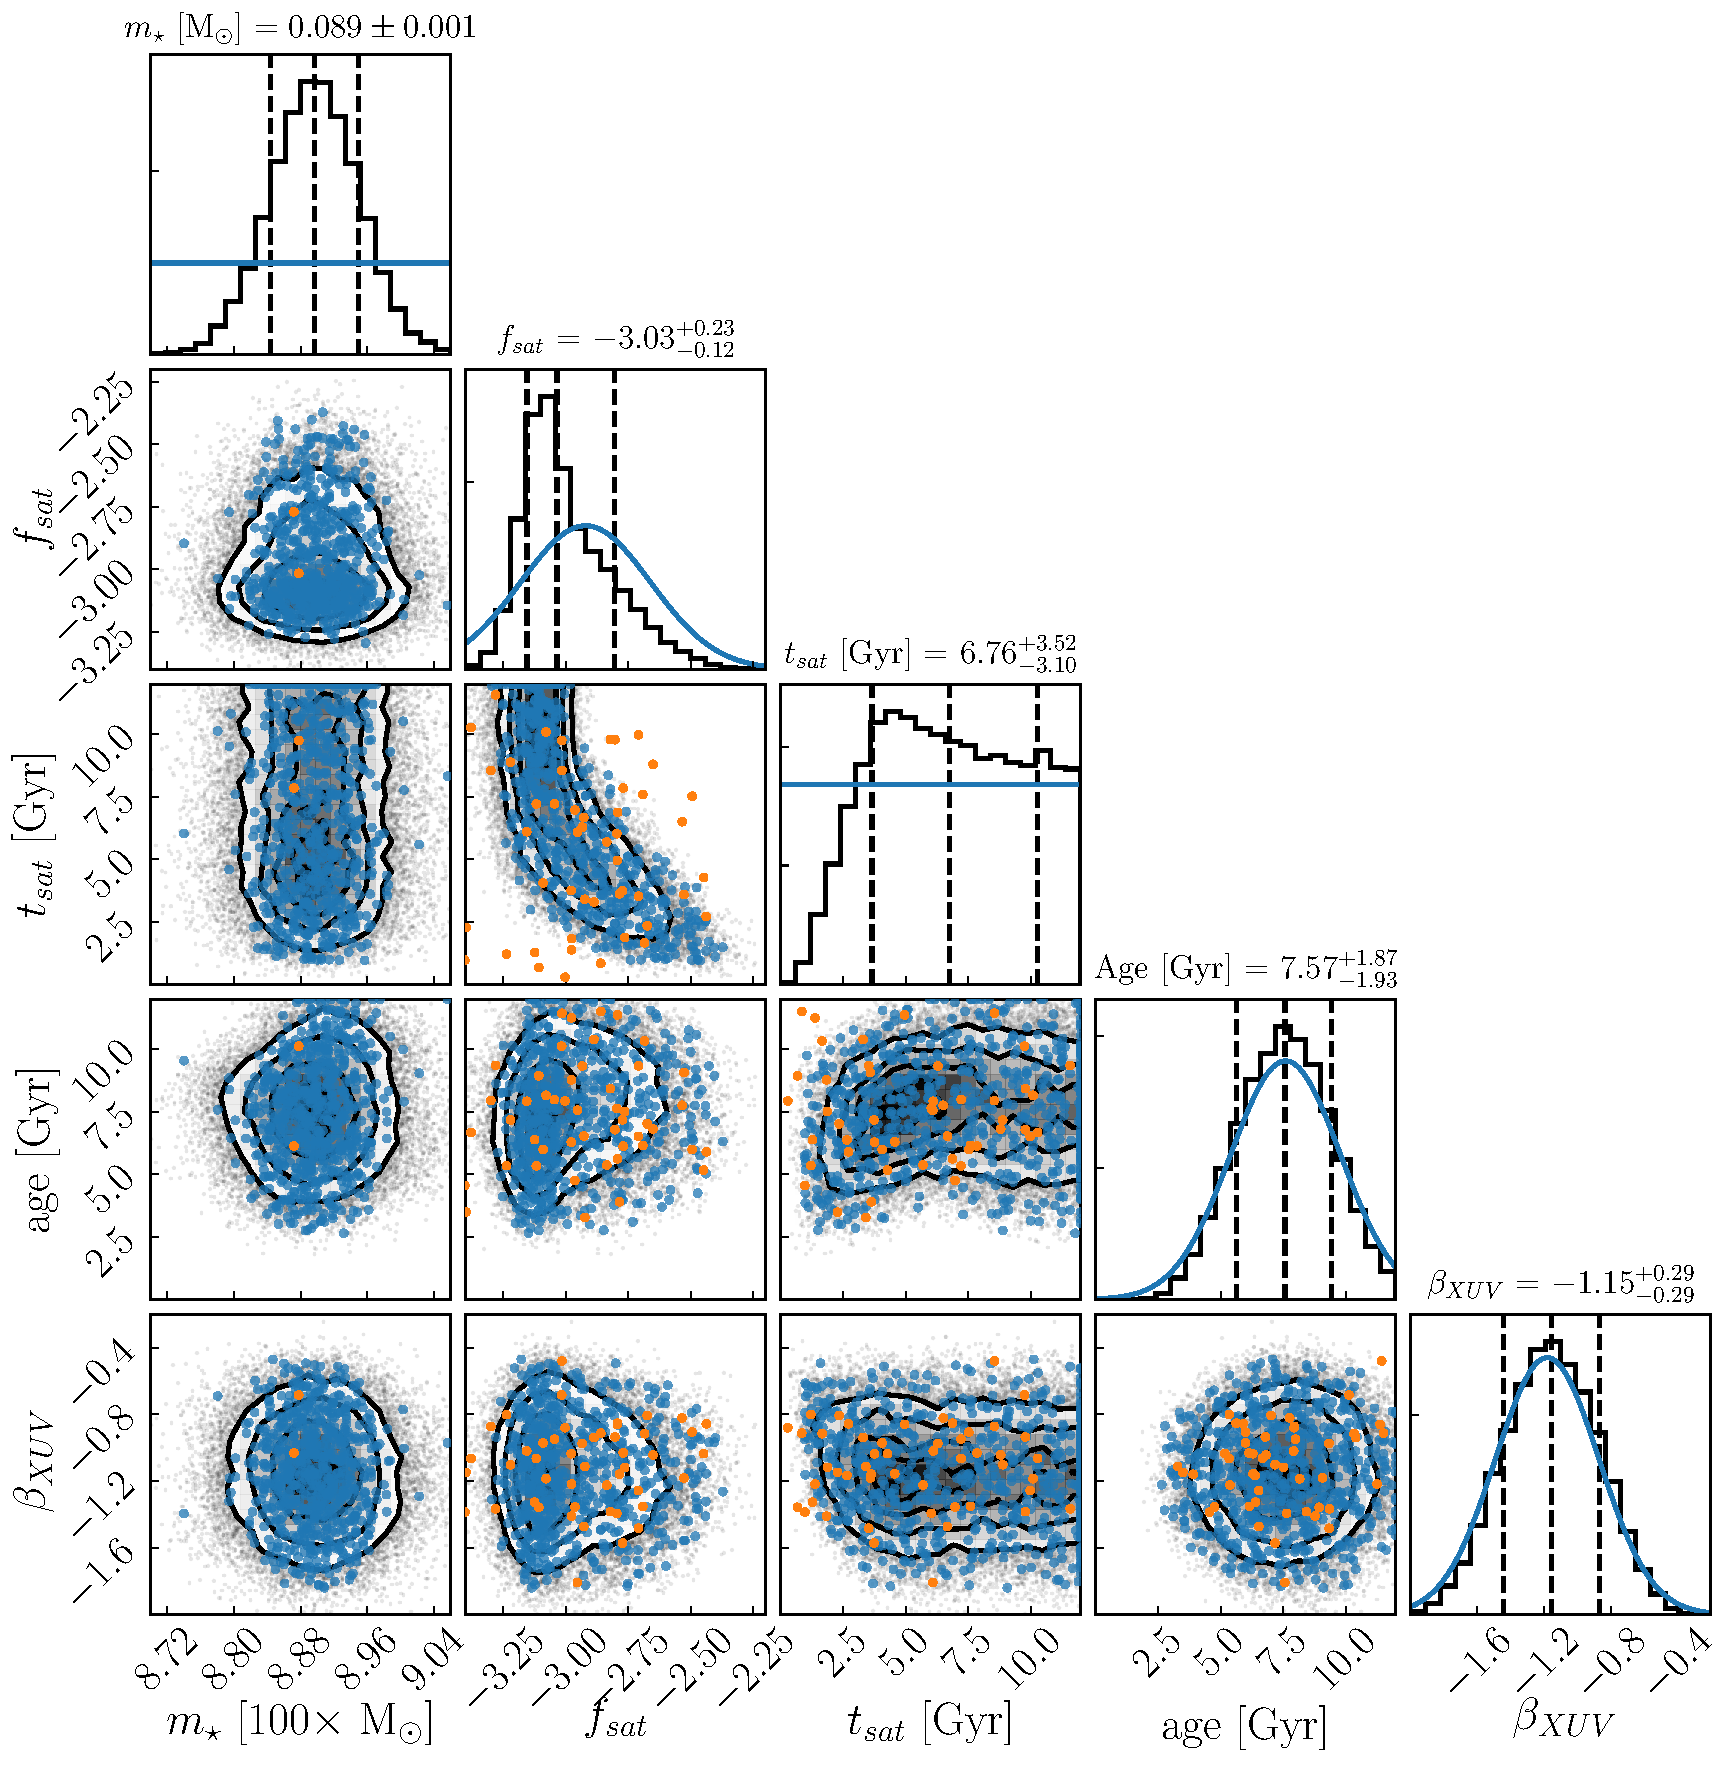
\includegraphics[width=\textwidth]{points.pdf}
   \caption{Same as Fig.~\ref{trap:fig:approx}, but overplotted with the training set for \approxposterior's GP. The orange points display the initial training points whereas the blue points display the points iteratively selected by maximizing the \citet{Kandasamy2017} utility function, Eqn.~(\ref{AP:eq:bape}). By design, \approxposterior selected points to expand its training set in regions of high posterior density, improving its GP's predictive accuracy in the most relevant regions of parameter space while seldom wasting computational resources in the low likelihood regions.}%
    \label{AP:fig:points}%
\end{figure}

As demonstrated in \citet{Kandasamy2017}, Eqn.~(\ref{AP:eq:bape}) identifies high-likelihood points where the GP's predictions are uncertain, significantly reducing the cost of training an accurate GP surrogate model. I found that Eqn.~(\ref{AP:eq:agp}) behaves similarly in practice. In Fig.~\ref{AP:fig:points}, I display the approximate joint and marginal posterior distribution derived by \approxposterior from \citet{Fleming2020} overplotted with the initial training set in orange and the points selected by sequentially maximizing Eqn.~(\ref{AP:eq:bape}) in blue. See Chapter 6 for additional information on the science underlying this application. Given the small initial training set, \approxposterior successfully selects high-posterior density points in parameter space to augment the GP's training set. Some points are selected in low-likelihood regions early on, typically near the edges of parameter space where the GP's uncertainty was initially large.

\subsection{Convergence} \label{AP:sec:app:convergence}

I assess the convergence of the \approxposterior algorithm by comparing the means of the approximate marginal posterior distributions over successive iterations. I consider an \approxposterior run ``converged" if the differences between the marginal posterior means, relative to the widths of the marginal posteriors, are less than a tolerance parameter, $\epsilon$, for $k_{max}$ consecutive iterations. Effectively, this criterion checks if the expected value of each model parameter over the posterior distribution varies by ${\leq}{\epsilon}$ standard deviations from the previous iteration's expected values. That is, I require the \approxposterior convergence diagnostic $z_{t,j}{\leq}{\epsilon}$ for all $j$, where
\begin{equation}
    z_{t,j} = |\mu_{t,j} - \mu_{t-1,j}| / \sigma_{t-1,j},
\end{equation}
 and $\mu_{t,j}$ and $\sigma_{t,j}$ are the mean and standard deviation of the approximate marginal posterior distribution for the $t^{th}$ iteration and the $j^{th}$ parameter. This quantity is analogous to the ``z-score" commonly used in many statistical tests. Following \citet{Wang2018}, I require this condition to be satisfied for $k_{max}$ consecutive iterations to ensure \approxposterior is producing a consistent result. With this scheme, \approxposterior tolerates deviations from the previous estimate that are less than, or at least consistent with, the previous values, given the inherent uncertainty implied by the width of the posterior distribution. For my application explored in Chapter 6, for example, I adopted conservative choices of $\epsilon = 0.1$ and $k_{max} = 5$. Each \approxposterior iteration, I also visually inspected the estimated posterior distribution to ensure convergence. 

In Fig.~\ref{AP:fig:convergence}, I display the convergence diagnostic quantity, $z_t$, as a function of iteration for each model parameter for the \approxposterior run presented in the Chapter 6 for illustrative purposes. In this case, \approxposterior quickly finds a consistent result as $z_t$ decreases below the convergence threshold within the first few iterations. For each parameter, $z_t$ continues to decrease until iteration 3 before stabilizing. The evolution of $z_t$ is not monotonic, however, owing to the stochastic nature of GPs, the hyperparameter optimization scheme, and MCMC sampling that can cause these values to occasionally be slightly worse than previous iterations. Requiring convergence over $k_{max}$ consecutive iterations mitigates the impact of this stochasticity.

\begin{figure}
\centering
	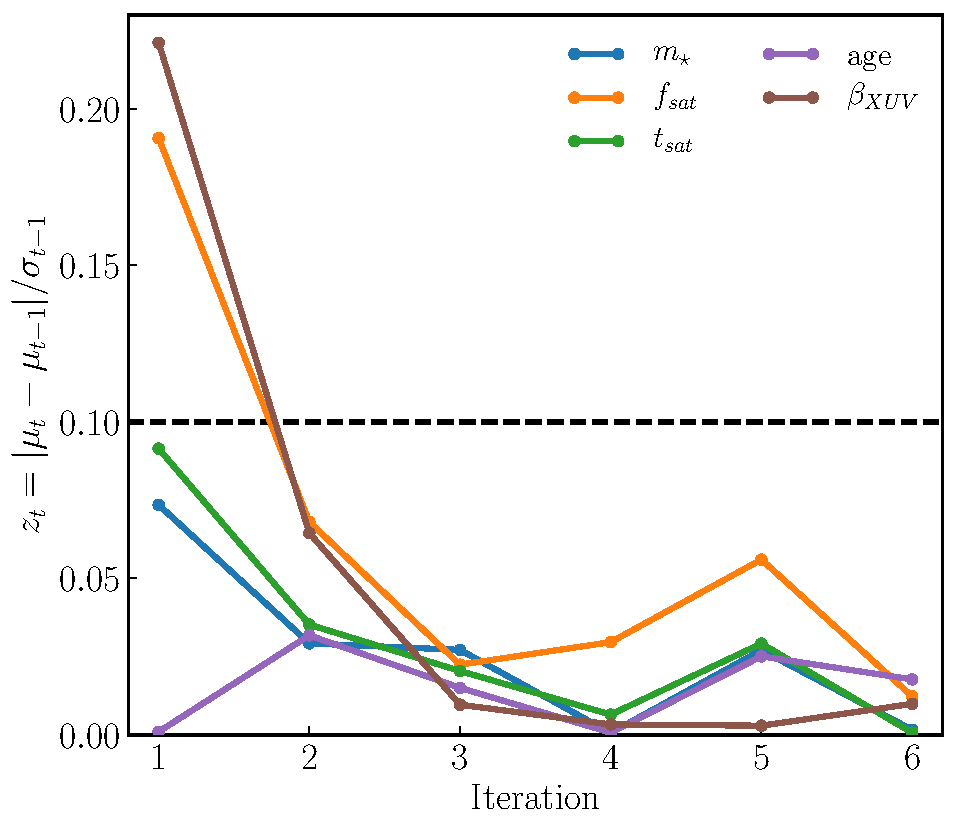
\includegraphics[width=\textwidth]{convergence.pdf}
   \caption{The \approxposterior convergence diagnostic, $z_t$, as a function of iteration for the run presented in the Chapter 6. Note that in \approxposterior, the initial iteration is iteration 0. The black dashed line indicates the adopted convergence threshold of $\epsilon = 0.1$. \approxposterior quickly converges to a consistent and accurate result.}%
    \label{AP:fig:convergence}%
\end{figure}

\subsection{A Simple Example} \label{AP:sec:example}

Here, I demonstrate how to use \approxposterior in practice to reproduce the 2-dimensional (2D) Rosenbrock function inference test examined by \citet{Wang2018}. The 2D Rosenbrock function is a classic optimization test function with a global minimum of 0 at (1,1). The Rosenbrock function exhibits non-linear, banana-like correlations making it a suitable challenge for \approxposterior. \citet{Wang2018} define the 2D Rosenbrock function likelihood as
\begin{equation} \label{AP:eqn:rosenbrock}
l(\textbf{x}) = \exp \left( -\frac{1}{100}(x_1 - 1)^2 - (x_1^2 - x_2)^2 \right)
\end{equation}
where $\textbf{x} = \{ x_1, x_2 \}$. In practice, \approxposterior works with the natural logarithm of Eqn.~(\ref{AP:eqn:rosenbrock}). I follow \citet{Wang2018} and adopt a uniform prior distribution for both $x_1$ and $x_2$ over [-5, 5].

Below, I include a simple Python script for applying \approxposterior to the 2D Rosenbrock inference problem.\footnote{The script is available at \href{https://github.com/dflemin3/approxposterior/blob/master/examples/inference/example.py}{https://github.com/dflemin3/approxposterior/blob/master/examples/inference/example.py}} In the first section, I define algorithm parameters that set the size of the initial training set, $m_0$, and control how \approxposterior operates, e.g. I only run two iterations by setting $n_{max} = 2$. As demonstrated below, this number of iterations is sufficient to reproduce the \citet{Wang2018} result. I also define the hard parameter bounds equal to the prior bounds to prevent the GP from blowing up by trying to learn in forbidden regions of parameter space, e.g. $x_1 > 5$. Next, I create the training set, $T = \{ \theta, y \}$, where the model parameters $\theta = \textbf{x}$. Note how $y$ is the sum of the lnlikelihood and lnprior distribution, that is, the unnormalized posterior probability. In \approxposterior notation, the GP iteratively learns $\hat{y} = \hat{f}(\textbf{x})$ as an approximation of $y = f(\textbf{x})$.

As explained above, \approxposterior requires a GP. \approxposterior has a handy convenience function for initializing GPs, \textit{defaultGP}, that creates a GP with a squared exponential kernel and takes care of various bookkeeping tasks for the user behind-the-scenes. In the script, I use this function to initialize the GP and pass it, along with functions that describe the lnlikelihood, lnprior, and how to sample from the prior to the \texttt{ApproxPosterior} object used to perform inference. Finally, I call the \approxposterior \texttt{run} method with the parameters described above and after a few minutes, the inference is complete. I finally extract the posterior samples using an \emcee utility function and visualize the joint posterior probability distribution estimated by \approxposterior. I display this distribution in Fig.~\ref{AP:fig:rosenbrock}. 

\inputpython{example.py}{1}{45}

Compare the posterior distribution in Fig.~\ref{AP:fig:rosenbrock} to Figures 1 and 3 from \citet{Wang2018}. The agreement is excellent, validating my implementation in \approxposterior. I also display the points selected by \approxposterior's training set augmentation procedure in red. As expected, the points \approxposterior selected preferentially cluster in regions of high posterior density, improving the accuracy of \approxposterior's GP surrogate model in the relevant regions of parameter space.

\begin{figure}
\centering
	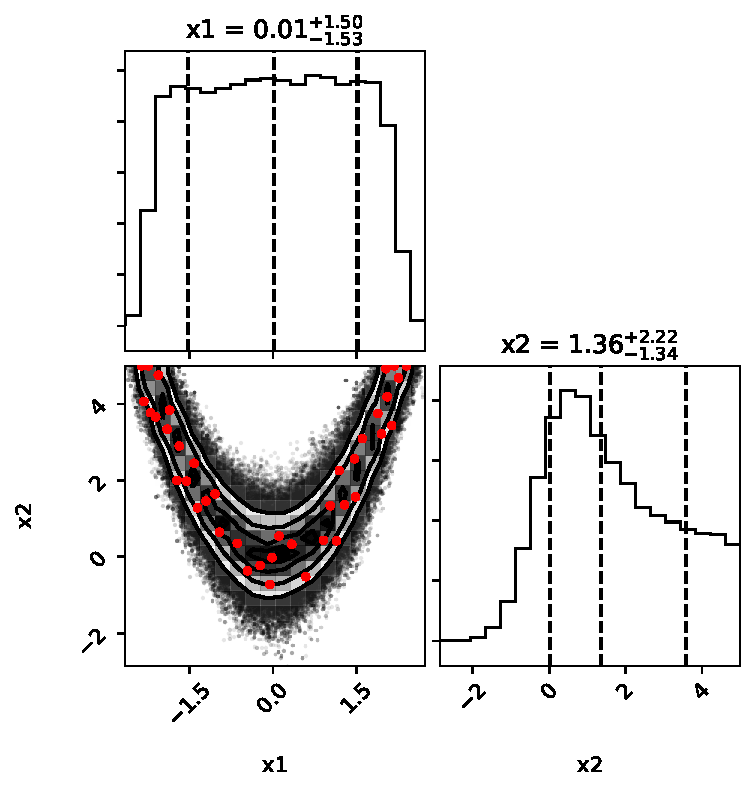
\includegraphics[width=\textwidth]{finalPosterior.pdf}
   \caption{The posterior probability distribution for the 2D Rosenbrock example from \citet{Wang2018} estimated by \approxposterior.  The red points denote points selected by \approxposterior's training set augmentation scheme using the BAPE algorithm. As explained above, \approxposterior preferentially selects points in regions of high posterior density. The posterior distribution estimated by \approxposterior is in good agreement with the results of \citet{Wang2018}, their Figures 1 and 3.}%
    \label{AP:fig:rosenbrock}%
\end{figure}

\subsection{Online Documentation} \label{AP:sec:docs}

I wrote extensive online documentation for \approxposterior that is located on both its main GitHub page\footnote{\href{https://github.com/dflemin3/approxposterior}{https://github.com/dflemin3/approxposterior}} and on an additional public documentation website\footnote{\href{https://dflemin3.github.io/approxposterior/}{https://dflemin3.github.io/approxposterior/}}. The online examples comprise both annotated Jupyter Lab notebooks and commented Python scripts, like the one shown above, to allow new users understand how \approxposterior is called and used in practice. Moreover, the online documentation includes the full \approxposterior API; each parameter in every \approxposterior class and function is fully described, including a definition for each parameter and reasonable default values. The online documentation serves to help new users employ \approxposterior in their own research. As the primary author of \approxposterior, I encourage new users to both fully read the online documentation and run all examples before developing scripts for their own application.

\section{Applying \approxposterior to Terrestrial Exoplanet Atmospheric Retrieval} \label{AP:sec:future}

\approxposterior is agnostic to the forward model it learns and is therefore not restricted to working with \vplanet-based lnprobabilities. \approxposterior is applicable for a wide array of Bayesian inference problems, particularly those that involve computationally-expensive models as demonstrated in this Chapter and in Chapter 6.  Here, I discuss an additional application of \approxposterior to the inference, or retrieval, of chemical abundances from synthetic transmission spectra of terrestrial exoplanet atmospheres (Lustig-Yaeger et al., in prep).

With future facilities like JWST eventually coming online, astronomers will likely be able to detect and characterize the first terrestrial exoplanet atmospheres. The most likely targets for this effort are the TRAPPIST-1 planets owing to the system's proximity to Earth, the relatively large planetary transit depths, and the small star-planet separations \citep{Gillon2016,Gillon2017,Morley2017,Lustig2019}. Since the TRAPPIST-1 planets all transit, JWST will be able to measure the absorption of stellar light passing though any atmosphere the planets possess as a function of wavelength, a technique known as transmission spectroscopy. Given suitable theoretical models for an exoplanet's transmission spectra, e.g. \citet{Lincowski2018}, modelers can solve the inference problem of inferring, or retrieving, the abundance of chemical species like O$_2$ in an exoplanet's atmosphere by matching theoretical models of transmission spectra with the observed spectra and uncertainties \citep[e.g.][]{KrissansenTotton2018,Tremblay2020}. Retrievals are another application of Bayesian inference, analogous to the case of matching \vplanet outputs with observational constraints discussed in this thesis.

Retrievals, however, are inherently computationally-expensive tasks because simulating transmission spectra requires not only simulating a physically-plausible exoplanet climate and atmospheric temperature structure \citep{Lincowski2018}, but also requires performing complex radiative transfer simulations \citep[e.g. with SMART, ][]{Meadows1996,Crisp1997}. To mitigate this computational expense, numerous groups have turned to machine learning to bypass this modeling in favor of training a model that maps atmospheric chemical abundances to transmission spectra using neural networks \citep{Waldmann2016,MarquezNeila2018,Zingales2018,Cobb2019,Fisher2019,Himes2020}. In this paradigm, the neural network is trained on a large ($\geq 10^4-10^5$) grid of pre-computed transmission spectra with known atmospheric chemical abundances and planetary properties. The neural network learns an approximate mapping between input planetary physical and atmospheric properties and the transmission spectra, bypassing complex climate and radiative transfer simulations to significantly reduce the computational expense of retrievals.

Although promising, neural network-based approaches suffer two related critical limitations. First, neural networks have a large number of parameters and hence require massive grids of pre-computed spectra for training whose size scales exponentially with the dimensionality of the inference. Simulating this initial grid is of course computationally-expensive. Second, if the theoretical model for the transmission spectra changes, say new line lists are developed or climate models are refined, the neural network's initial training grid must be recomputed as a previously-trained neural network would have been tuned to out-dated, or at worst, incorrect physics, biasing any retrieved abundances. 

Here, I present work-in-progress from Lustig-Yaeger et al, in prep, to demonstrate that \approxposterior is well-suited to retrievals, providing comparable accuracy as direct inference methods but requiring about 800 times fewer computational resources. I consider the case of inferring the isothermal atmospheric temperature and mixing ratios of H$_2$O and CO$_2$ from a synthetic transmission spectra of TRAPPIST-1e with noise levels comparable to what astronomers expect from JWST \citep{Lincowski2018}. In this case, I consider two retrieval methods (see Lustig-Yaeger et al, in prep. for a complete description). For the first method, I run SMART radiative transfer simulations each $\textbf{x}$ evaluation within an \emcee sampler to derive the posterior distribution. I refer to this method as the ``fiducial" inference method. For the second, I use \approxposterior within \emcee to replace the $\textbf{x}$ evaluation and estimate the posterior distribution. Each method's MCMC chain were ran with identical parameters. 

I display the posterior distributions inferred by both methods in Fig.~\ref{AP:fig:comparison}. The fiducial posterior distribution is purple and the \approxposterior-derived distribution is orange. Both the joint and marginal posterior distributions derived by \approxposterior are in excellent with the distributions derived by the fiducial method, demonstrating \approxposterior's ability to accurately replace the complex radiative transfer simulations for computing the lnprobability. Note the how the marginal constraints, both the best fit value and the uncertainties, derived by both methods listed in Fig.~\ref{AP:fig:comparison} are in nearly perfect agreement. Furthermore, \approxposterior required about 4,000 SMART simulations total to train its GP whereas \emcee required about 3,000,000 to evaluate the MCMC. In this case, \approxposterior is about ${\sim}800$ times more efficient than the fiducial method, a dramatic reduction in computational cost without appreciably reducing the accuracy on the inference. Clearly, \approxposterior offers a promising method to enable rapid and accurate Bayesian inference for computationally-expensive models.

\begin{figure}
\centering
	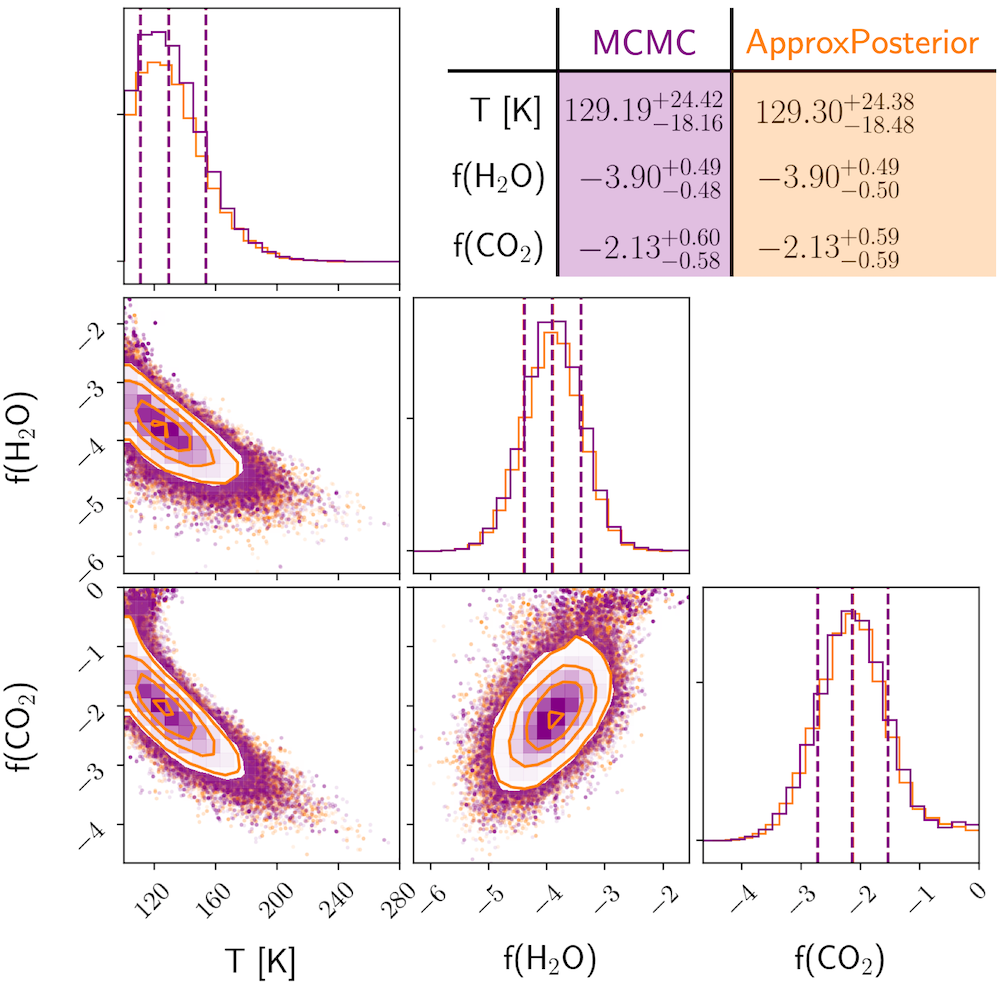
\includegraphics[width=\textwidth]{emceeAPComparison.png}
   \caption{Joint and marginal posterior probability distributions derived by \emcee (purple) and \approxposterior (orange) from an atmospheric retrieval of a simulated noised JWST transmission spectrum of TRAPPIST-1e (used with permission from Lustig-Yaeger et al., in prep). This retrieval experiment attempts to infer the isothermal atmospheric temperature, $T$, and the mixing ratios of H$_2$O and CO$_2$. \approxposterior accurately recovers both the nontrivial correlations between model parameters and marginal parameter constraints as did \emcee, within Monte Carlo error, but requiring about 800 times fewer computational resources.}%
    \label{AP:fig:comparison}%
\end{figure}

\section{Conclusions}

In this Chapter, I introduced \approxposterior, an open-source Python machine learning package that uses GP regression for rapid and accurate approximate Bayesian inference. I outlined the mathematics and algorithm underpinning \approxposterior and examined its practical application. After explaining the \approxposterior algorithm and convergence scheme, I sketched an in-progress research project using \approxposterior and demonstrated that it was as accurate as direct inference methods using \emcee, but required 800 times fewer computational resources. 

